\documentclass{standalone}

\usepackage{amsmath,amssymb,amsthm}
\usepackage{tikz}
\usetikzlibrary{positioning,decorations.pathreplacing,quotes}

\begin{document}

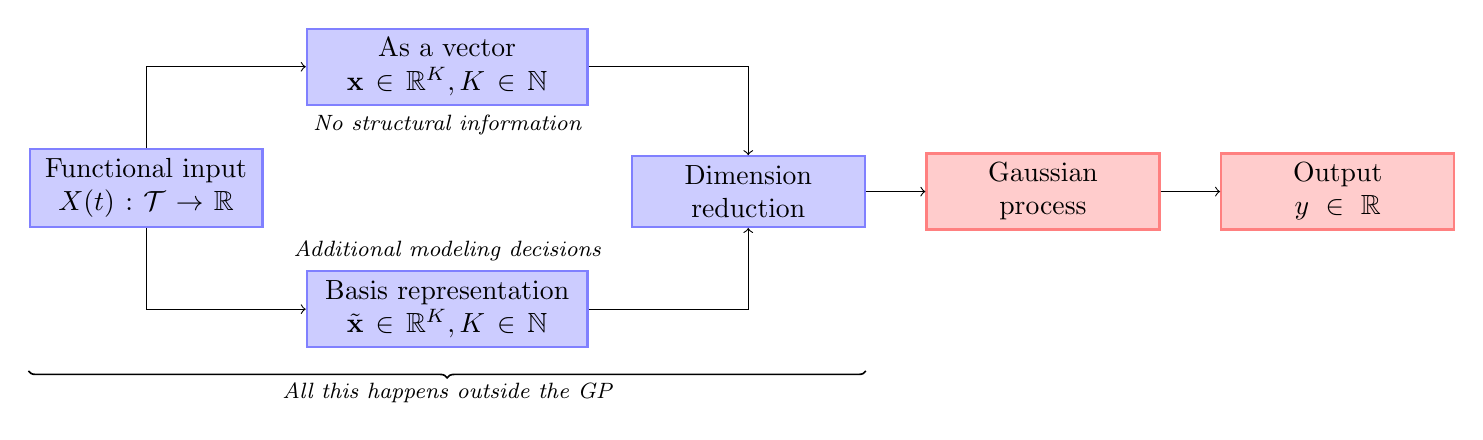
\begin{tikzpicture}
  [
  txtbox1/.style={rectangle,align=center,draw=blue!50,fill=blue!20,thick},
  txtbox2/.style={rectangle,align=center,draw=red!50,fill=red!20,thick},
  every label/.style={font=\itshape\footnotesize}
  ]

  \node (inp)  [txtbox1] at ( 0,  0) [text width=18ex] {
    Functional input \\ $X(t): \mathcal{T} \to \mathbb{R}$
  };
  \node (vec1) [txtbox1] [above right=5ex of inp]   [text width=22ex]
  [label=below:No structural information]{
    As a vector \\ $\mathbf{x} \in \mathbb{R}^K, K \in \mathbb{N}$
  };
  \node (vec2) [txtbox1] [below right=5ex of inp]   [text width=22ex]
  [label=above:Additional modeling decisions]{
    Basis representation \\ $\tilde{\mathbf{x}} \in \mathbb{R}^K, K \in \mathbb{N}$
  };
  \node (dred) [txtbox1] [above right=5ex of vec2] [text width=18ex]
  {
    Dimension \\ reduction
  };
  \node (gp)   [txtbox2] [right=5ex of dred] [text width=18ex] {
    Gaussian \\ process
  };
  \node (out)  [txtbox2] [right=5ex of gp] [text width=18ex]  {
    Output \\ $y \in \mathbb{R}$
  };
  \node [below=7ex of vec2.north, label=below:All this happens outside the GP] {
  };
  \draw [->] (inp.north) |- (vec1.west);
  \draw [->] (inp.south) |- (vec2.west);
  \draw [->] (vec1.east) -| (dred.north);
  \draw [->] (vec2.east) -| (dred.south);
  \draw [->] (dred.east) -- (gp.west);
  \draw [->] (gp.east)   -- (out.west);
  \path (inp.south west)
  edge[decorate,decoration={brace,mirror,raise=12ex},line width=.6pt]
  (inp.south west -| dred.south east);
\end{tikzpicture}

\end{document}

%%% Local Variables:
%%% mode: latex
%%% TeX-master:
%%% End:
